% THIS IS SIGPROC-SP.TEX - VERSION 3.1
% WORKS WITH V3.2SP OF ACM_PROC_ARTICLE-SP.CLS
% APRIL 2009
%
% It is an example file showing how to use the 'acm_proc_article-sp.cls' V3.2SP
% LaTeX2e document class file for Conference Proceedings submissions.
% ----------------------------------------------------------------------------------------------------------------
% This .tex file (and associated .cls V3.2SP) *DOES NOT* produce:
%       1) The Permission Statement
%       2) The Conference (location) Info information
%       3) The Copyright Line with ACM data
%       4) Page numbering
% ---------------------------------------------------------------------------------------------------------------
% It is an example which *does* use the .bib file (from which the .bbl file
% is produced).
% REMEMBER HOWEVER: After having produced the .bbl file,
% and prior to final submission,
% you need to 'insert'  your .bbl file into your source .tex file so as to provide
% ONE 'self-contained' source file.
%
% Questions regarding SIGS should be sent to
% Adrienne Griscti ---> griscti@acm.org
%
% Questions/suggestions regarding the guidelines, .tex and .cls files, etc. to
% Gerald Murray ---> murray@hq.acm.org
%
% For tracking purposes - this is V3.1SP - APRIL 2009

\documentclass{acm_proc_article-sp}
%\usepackage{hyperref}
\usepackage{multirow}

\begin{document}

\title{A Biomechanical Approach to Biped Dynamics}
%
% You need the command \numberofauthors to handle the 'placement
% and alignment' of the authors beneath the title.
%
% For aesthetic reasons, we recommend 'three authors at a time'
% i.e. three 'name/affiliation blocks' be placed beneath the title.
%
% NOTE: You are NOT restricted in how many 'rows' of
% "name/affiliations" may appear. We just ask that you restrict
% the number of 'columns' to three.
%
% Because of the available 'opening page real-estate'
% we ask you to refrain from putting more than six authors
% (two rows with three columns) beneath the article title.
% More than six makes the first-page appear very cluttered indeed.
%
% Use the \alignauthor commands to handle the names
% and affiliations for an 'aesthetic maximum' of six authors.
% Add names, affiliations, addresses for
% the seventh etc. author(s) as the argument for the
% \additionalauthors command.
% These 'additional authors' will be output/set for you
% without further effort on your part as the last section in
% the body of your article BEFORE References or any Appendices.

\numberofauthors{1} %  in this sample file, there are a *total*
% of EIGHT authors. SIX appear on the 'first-page' (for formatting
% reasons) and the remaining two appear in the \additionalauthors section.
%
\author{
% You can go ahead and credit any number of authors here,
% e.g. one 'row of three' or two rows (consisting of one row of three
% and a second row of one, two or three).
%
% The command \alignauthor (no curly braces needed) should
% precede each author name, affiliation/snail-mail address and
% e-mail address. Additionally, tag each line of
% affiliation/address with \affaddr, and tag the
% e-mail address with \email.
%
% 1st. author
\alignauthor
Geoyeob Kim\\
       \affaddr{Department of Computer Science}\\
       \affaddr{KAIST, Daejeon, Korea}
       \email{gasbank@naver.com}
}
% There's nothing stopping you putting the seventh, eighth, etc.
% author on the opening page (as the 'third row') but we ask,
% for aesthetic reasons that you place these 'additional authors'
% in the \additional authors block, viz.

\date{16 December 2010}
% Just remember to make sure that the TOTAL number of authors
% is the number that will appear on the first page PLUS the
% number that will appear in the \additionalauthors section.

\maketitle
\begin{abstract}
Adopting physically-based dynamics model for synthesizing character animation is widely used.
Since most concepts of dynamics and physical simulation came from robotics and mechanical engineering,
biped models used in character animation also took a form of robots.
The robot-like biped models have actuated joint motors in their respective joints,
so that the motors are controlled to rotate bodies to make desired poses.

We present a new biped model based on the biomechanical idea that human movements are occurred
by controlling muscle fibers attached to skeletal structures instead of actuated motors on joints.
Also an optimization-based tracking control scheme for walking and balancing using our model is introduced.
By changing muscle fiber parameters and constraints, various human motions are synthesized.
\end{abstract}

% A category with the (minimum) three required fields
\category{I.3.7}{Computer Graphics}{Three-Dimensional Graphics and Realism}[animation]
%A category including the fourth, optional field follows...
%\category{D.2.8}{Software Engineering}{Metrics}[complexity measures, performance measures]

\terms{Theory}


\keywords{character animation, physical simulation, biomechanics}
%\keywords{ACM proceedings, \LaTeX, text tagging} % NOT required for Proceedings

\section{Introduction}
Being an essential component for animations and video games,
bipedal character animation techniques have drawn much attention from
both academia and industry. Physically-simulated approaches have been
adopted to synthesize realistic and physically correct motions
automatically instead of relying on labor-intensitve key-frame animation
techqniues. In these approaches, a character is designed and controlled
as a consistent dynamic model, being represented as an articulated
figure. This model consists of a set of body segments, each being
considered as a rigid body, and joints connecting these segments.
This kind of models is used widely due to their adquacy to formulating
the Lagrangian equations of motion using the generalized coordinates
which simplifies motion description.
The joints used in the model are considered as ideal rigid joints,
that is, each of them connects the two rigid bodies with a certain DOFs.
Typically, translational DOFs are not treated in joints to disallow a dislocation of bones.
For example, hinge joints with one DOF are used at knees or elbows and
ball joints with three DOFs are used at hips. Actuation on the joints
changes their respective DOFs. Thus it is natural to call this kind of joints
\emph{actuated motor joints}. Motions can be created by
controlling these motor joints properly. In robotics this approach is
commonly adopted. The main interest of creating motions
with a dynamics model is focused on how to design the motor joint controllers.

The concept of actuated motor joints is unrealistic in the perspective of
biomechanics. No human being has that kind of motors in their joints.
Humans control their legs or arms by pulling bones using attached
muscles. Although the whole mechanism is quite complicated,
the structure of human muscle fibers is well-known, and biomechanical
results are availble concerning the most basic human actions
such as walking and jumping \cite{citeulike:2547705, citeulike:7093575}.

This thesis presents a biomechanical approach to biped dynamics. We
introduces muscle fibers as the only actuating elements
of the biped and get rid of all rigid motor joints in the previous biped
models. Consequently, joints are not rigid anymore in our approach.
We use ligaments in the place of joints
to hold the bodies firmly but not rigidly. This substitution
simulates human cartilages, which provide a shock absorption
system to sustain stability when external or internal disturbances exist \cite{shock}.
We control the rigid bodies with muscle fibers each of which are modeled as
a spring-damper system. Every muscle fiber has a linear actuator and
motions are created by controlling the actuator. Instead of controlling
the bodies with motor joints, it is highly effective in energy consumption
since torques are created more easily by pulling the bones with a muscle
fiber which lie at a distant place from an axis of rotation.

Besides the muscle-actuated character model we adapt the concept of
human gait phases to control biped locomotion. Human gait analysis is an extensively
studied area, and deals with the mechanism of human locomotion
by throughly experimenting and measuring subjects.
A human walking cycle consists of a sequence of phases, each of which has
its own objective and features.
In computer animation, such biomechanical research results have not fully exploited yet.
Previous approaches rely on optimization-based
techniques such as a motion tracker with a linear quadratic regulator (LQR)
or a quadratic programming optimizer and concentrate on the high level
objectives such as minimizing the actuation force or following the reference
trajectory without considering how human being tries
to achieve it biomechanically. For instance, in our model, a set of muscle fibers is
actuated according to a certain gait phase and the other fibers remain
unactuated to utilize its passive energy while prevalent approaches blindly seek
this kind of the natural human behavior with the macroscopic objectives.
Although seemingly having succeeded for generating nice-looking motion,
they can be enhanced by introducing biomechanical knowledge into both
a dynamics model and an optimization scheme.

\section{Related work}
Designing and controlling a physically simulated character is a long-standing
challenge in robotics and computer graphics. A physically
synthesized motion that actively responds to the environment is quite
promising because it is hard to keyframing a natural animation for every motion
manually. Although the combination of motion capture data and manual keyframing
shows a quality of motion, it is not straightforward to make a character
interacts with its environment if a pre-recorded motion clip is used.
By adapting physical simulation into a character animation we can overcome
this issue. The problem is that still there is no ultimate solution for controlling
a simulated character motion.

Some approaches proposed a controller which is based on the fact
that the ground reaction forces or contact forces affect the global
DOFs of the character significantly \cite{SCA07:249-258:2007, journals/tog/MuicoLPP09}.
Muico and his colleagues
presented a contact-aware controller \cite{journals/tog/MuicoLPP09}.
The approach is
heavily based on the theory of optimal control \cite{lewis}.
They modified the LQR to consider the presence of the ground reaction forces.
We also take the contact forces into account but in a different way.
The estimated contact forces are calculated using a linear complementarity
problem (LCP) before any actuation applied. The actuation force is then
determined with the consideration of the estimated contact forces.

Using an optimization technique for biped control is relatively complicated method.
There exists a simpler way to control. KangKang Yin and her colleagues
presented a simple proportional-derivative (PD) control framework \cite{journals/tog/YinLP07}.
They used a finite state machine (FSM) in which target poses are defined
for each state. Compared to the complexity of dynamics model,
the structure of controller is simple and robust to external disturbances.
Since they do not consider energy efficiency or passive forces during
simulation, the animation shows some stiff behavior.
Even if we can get more elaborate animations by increasing
the number of states in the FSM, it is not practically possible since the
number of parameters is proportional to the number of states.

Optimization-based approaches shown to be a good way to address many challenges
in biped control such as high dimensionality, underactuated-ness and
nonlinearity. Most of work set up their goal to determine the joint
torques to make a desired pose or a sequence of desired poses.
Instead of finding joint torques, Jain and his colleagues formulated
an optimization problem which finds joint angles directly \cite{Jain:09:OIM}. The joint torques
are implicitly calculated during the optimization process. The advantage of
this approach is that it is easy to design various types of objectives such as
moving a hand to nearby wall or placing a swing foot to some place while it
is not intuitive to formulate with torque-based optimization techniques.

%------%

Our goal is not so different from these work. However these work mainly focused
on the controller design and not the character model itself. Our work is
partly relies on the idea stuided in the field of biomechanics.
Some researchers in biomechanical engineering focus on the movement
disorder and the biomedical applications such as artificial joints.
There are abundant work exist which use a model similar to
a real human body since it is important to study the mechanism of underlying
structure of human body in that area \cite{vr-305}. Thelen and his colleagues
illustrated
the algorithm to compute muscle excitation patterns that produce
coordinated movements of muscle-actuated dynamic models \cite{Thelen2003321}.
They simulated
a pedaling motion while fixing the upper body to investigate the excitation
pattern of 30 muscle fibers which significantly affecting leg movements.

Liu and her colleagues tried to exploit the passive characteristics of
muscle fiber by including a torsion spring in joints \cite{Liu:2005:LPB}.
However, the actuation
is still occurred by joint motors and the muscle fibers are not explicitly used.

The action for each muscle groups can be anticipated by adopting the
fact regarding to gait phases \cite{perry}. The gait phases are the essential component
when analyzing a person's walking pattern. It directly identifies the
functional significance of the different motions occurring at the
individual joints. While controlling the character we
can determine the current gait phase. For each gait phase,
a set of muscle fibers from the entire muscles is selected to be actuated
and the others will be unactuated. This approach will give us an explicit
way to make full use of passive energy.

%The muscle fiber model we use is composed of two springs and a damper.
%This simple muscle model is explained in detail in the supplementary
%documents [SHADMEHR]. In the document they assume that spring stiffness constants
%and viscosity of the damper are constants. Some studies suggest that animals
%vary stiffness according to the specific locomotion task.[FARLEY]
%Since the model consists of springs we definitely need rest lengths for that
%springs. However rest lengths are not simply defined on real muscles.
%[...]

\section{Problem definition}

We model a character which consists of rigid bodies and virtual muscle fibers.
With this biomechanical model we design a reference trajectory tracker.
Specifically we build the equations of motion which have the
form of
\begin{equation}\label{MoEq}
\mathbf{M}(\chi)\ddot\chi + C(\chi,\dot\chi ) = f_g(\chi) + f_c(\chi, \dot\chi, \tau ) + \tau (\chi, \dot\chi, u)
\end{equation}
where $\mathbf{M}$ is a generalized mass matrix and $\chi$ is a generalized
linear and angular position
state vector and $\dot\chi$, $\ddot\chi$ are its first and second time derivatives,
respectively. $C$ represents Coriolis and centrifugal forces.
$G$ and $f_c$ represents gravitational forces and contact forces.
$\tau$ and $u$ denotes muscle tension and actuation forces.
For the case of a freely moving single
rigid body with 6-DOF, $\mathbf{M}$ will be $6\times 6$ matrix and $\chi$,
$f_c$, $\tau$, $C$ and $G$ will be a 6-dimensional vector. The dimension of $u$ is
determined by the number of muscle fibers. We have control
over none of the variables such as $\chi$, $\dot\chi$, $\ddot\chi$ and $f_c$.
$f_c$ is uncontrollable because it is the ground reaction force. This means that
$f_c$ is a reaction force arises by pushing the ground with the character's feet.
The only way to change $\chi$ to a certain desired value is done by controlling $u$
properly. If we denote a reference position and velocity from motion capture data
as $\bar\chi$ and $\dot{\bar\chi}$, \eqref{MoEq} can be more elaborated
to reveal its structure as a tracker:
\begin{equation}\label{MoEq2}
\mathbf{M}(\chi)\ddot\chi + C(\chi,\dot\chi ) = f_g(\chi) + f_c(\chi, \dot\chi, \tau ) + \tau (\chi, \dot\chi, \bar\chi, \dot{\bar\chi}).
\end{equation}
Note that the muscle actuation force $u$ is calculated in $\tau$ internally.

Unfortunately, $C$, $f_c$ and $\tau$ are highly nonlinear functions of the current state and the
actuation forces, it is hard to figure out the actuation forces which attain
the desired acceleration of the system. To make matters worse, $f_c$ is the function
of muscle forces $\tau$, it is extremely difficult or even impossible
to solve \eqref{MoEq2} for the function of $\tau$ or $u$ in a closed-form
equation.
To make the problem tractable, we make a few assumption.

Because we represent times as discrete samples, all the functions of
time-varying variables need to be represented in a discrete domain.
We discretize the time into samples with small intervals $h$. We define
the velocity $\dot\chi^{(l)}$ and the acceleration $\ddot\chi^{(l)}$, at current
time sample $l$, by backward and central finite differences, respectively.
\begin{align}
\dot\chi^{(l)}  \equiv {} & \frac{\chi^{(l)}-\chi^{(l-1)}}{h}\label{vel-dis}\\
\ddot\chi^{(l)} \equiv {} & \frac{\chi^{(l+1)}-2\chi^{(l)}+\chi^{(l-1)}}{h^2}\label{acc-dis}
\end{align}

\section{Algorithm}

Given motion capture data for human locomotion, we classify the motion
sequence automatically into respective phases. For each phase,
an optimization formulation is built to calculate muscle actuation forces
of our biped model. The actuated and unactuated muscles are explicitly configured
with respect to a corresponding phase.

\begin{figure}[h!]
  \centering
  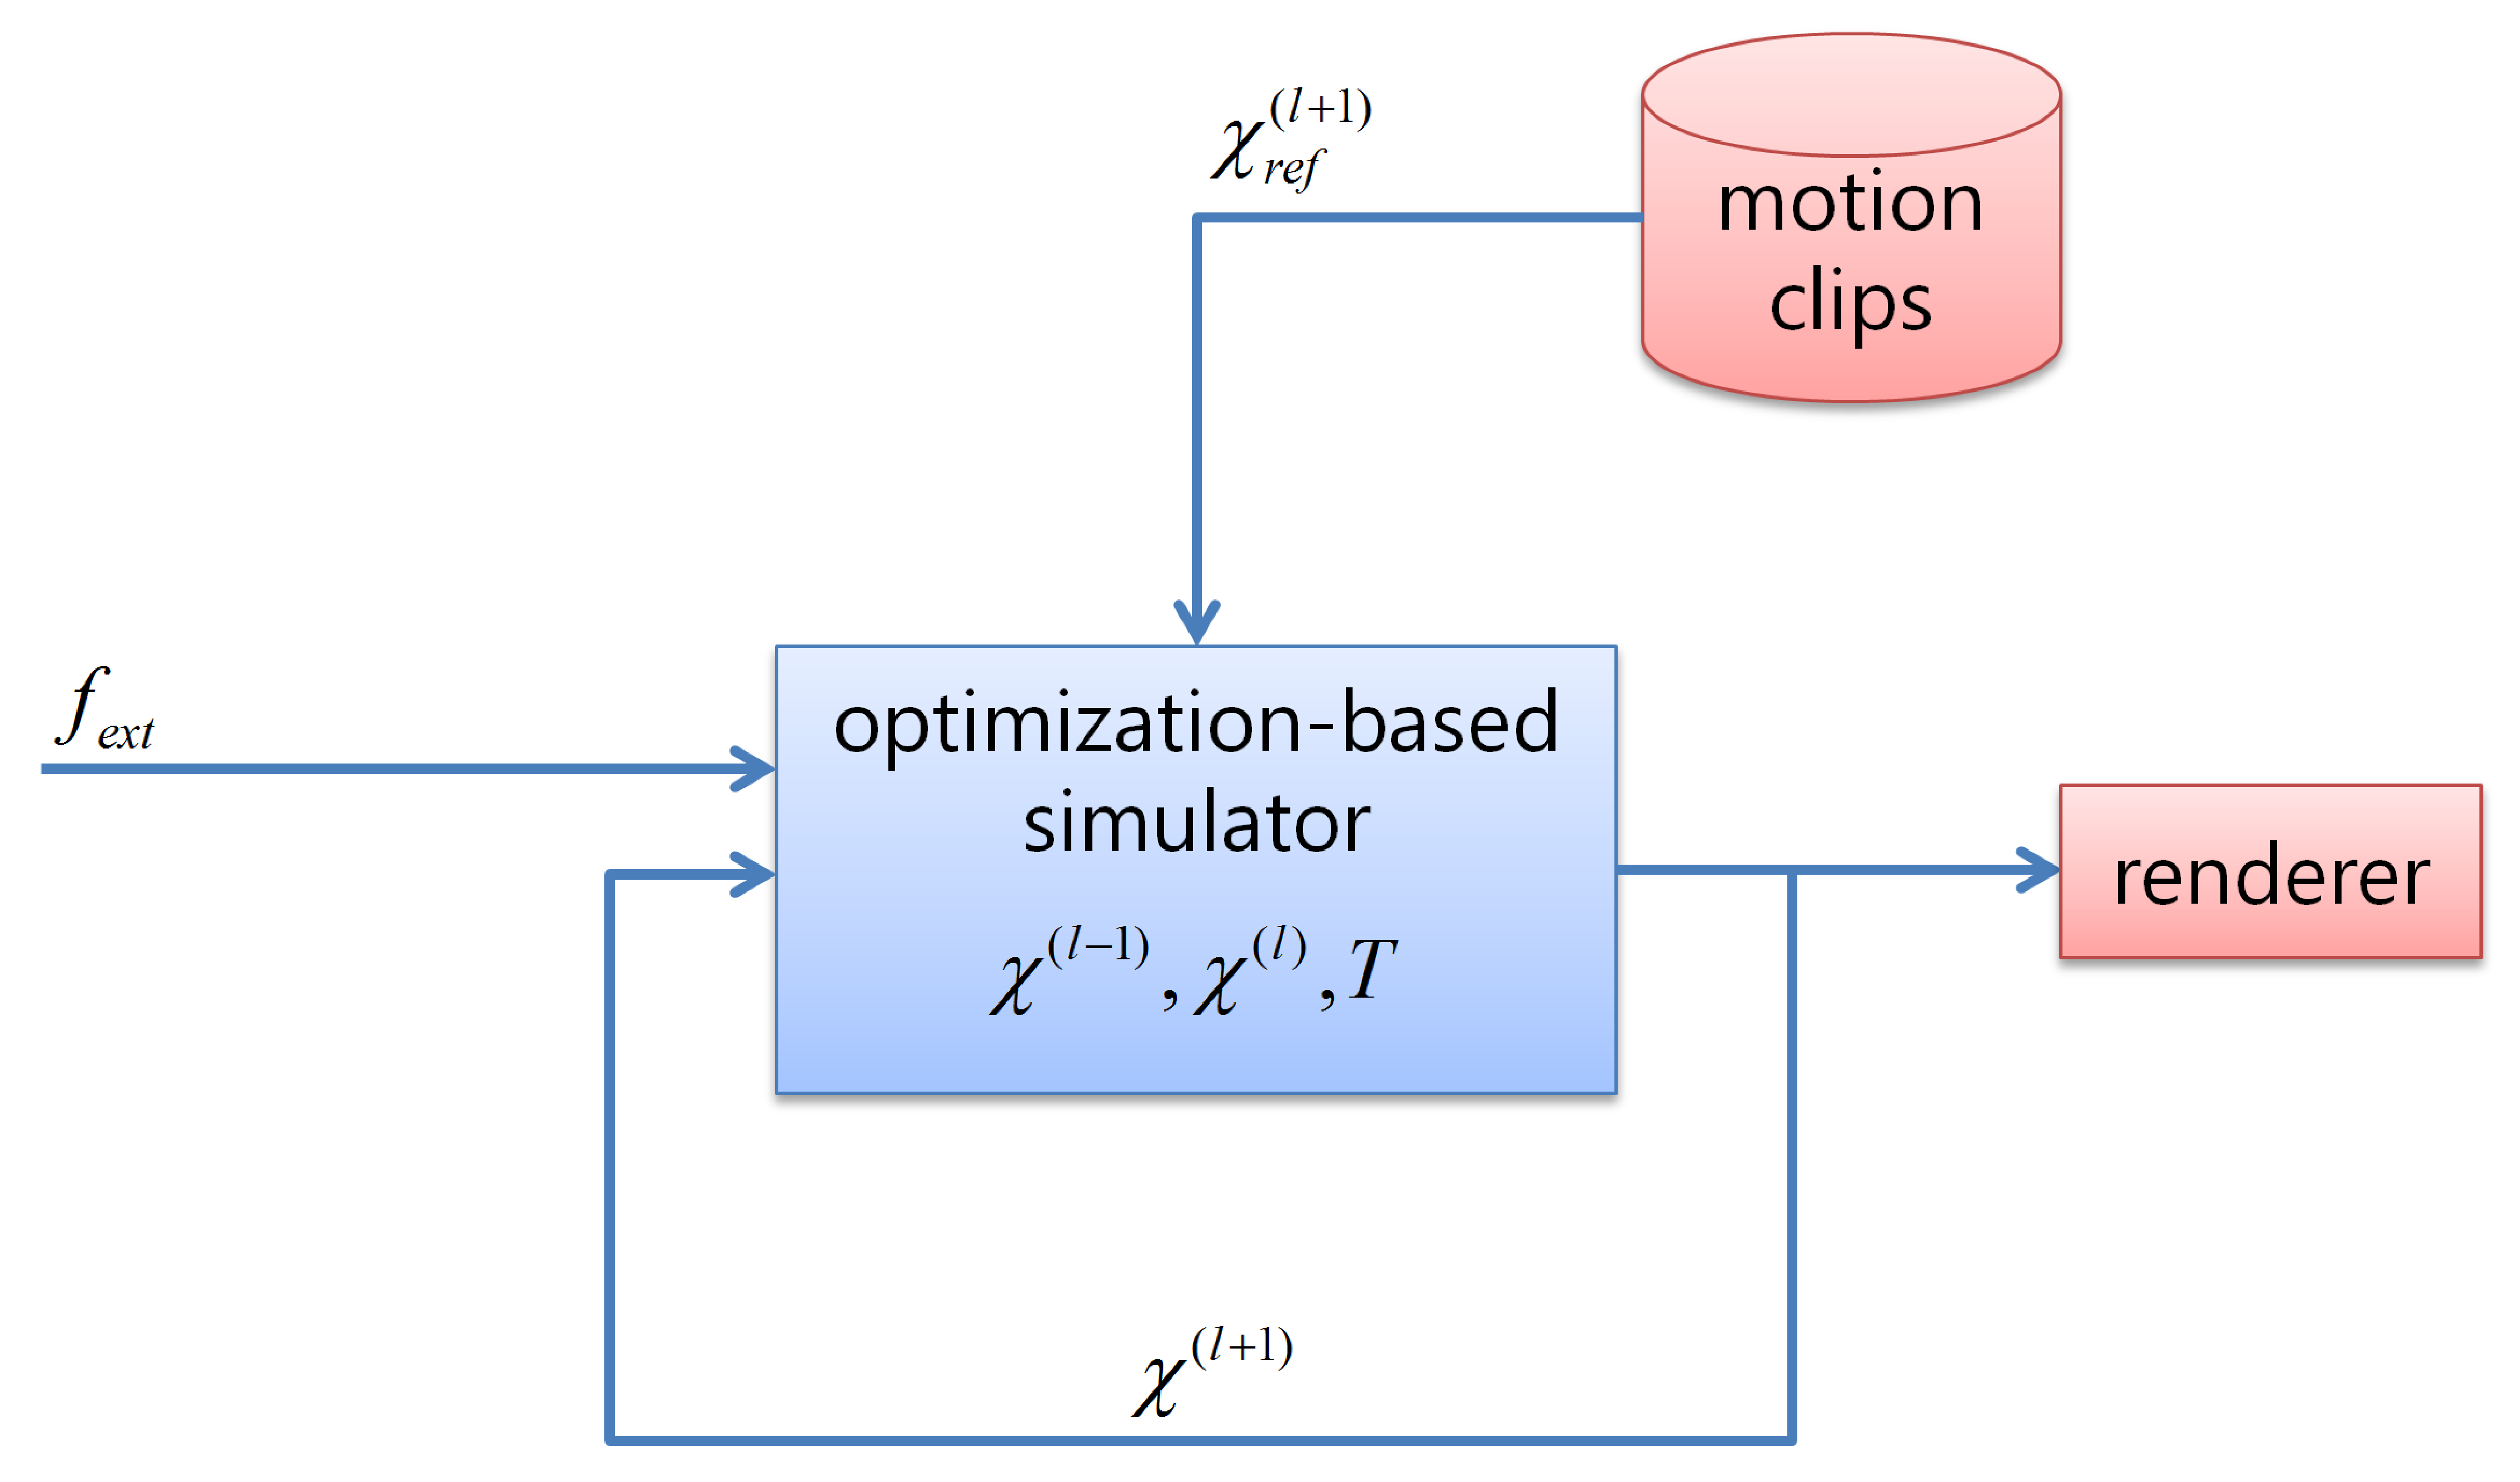
\epsfig{file=overview.eps, width=3in}
  \caption{Algorithm overview diagram}
\end{figure}


\subsection{Rigid body dynamics}

The concept of rigid body is commonly used in a physically-simulated
character model.
Our character model is a full four-limbed biped, which consists of 14 rigid bodies.
The forward dynamics algorithm gives the following equation:
\begin{equation}
\ddot\chi =\mathbf{M}^{-1}(\chi) ( \tau - C(\chi,\dot\chi) ).
\end{equation}

We define a discrete-time state vector $Y$. For brevity, we use $Y^{(l)}$
to indicate a discrete-time value of $Y$ at $l$-th time step $Y(t_l)$.
We use an explicit Euler integration
scheme using both $Y$ and the equations of motion to derive a complete
forward dynamics formulation.
\begin{equation}
Y^{(l)} =
\left[ {\begin{array}{cc}
 \chi^{(l)}   \\
 \dot\chi^{(l)}   \\
 \end{array} } \right]
\end{equation}
\begin{align}
f(Y^{(l)})=\dot{Y}^{(l)}
 &=
\left[ {\begin{array}{cc}
 \dot\chi^{(l)}   \\
 \ddot\chi^{(l)}   \\
 \end{array} } \right] \notag\\
 &=
\left[ {\begin{array}{cc}
 \dot\chi^{(l)}   \\
 \mathbf{M}^{-1}(\chi^{(l)}) ( \tau^{(l)} - C(\chi^{(l)},\dot\chi^{(l)}) )   \\
 \end{array} } \right]
\end{align}
\begin{equation}
Y^{(l+1)}=Y^{(l)}+hf(Y^{(l)})
\end{equation}
Note that we need the position and velocity values of a certain time step
to store the state because the equations of motion for rigid bodies
are the second order differential equations.
If we model a dynamics system
which can be expressed by the first order differential equations of motion
then we need only a position as the state vector.



As stated in the previous section most of the existing work on
character animation used an articulated body to represent a character.
In the articulated body each body is connected to another body with
various types of joints. Since we use no joint at all in the character
model the mathematics involved in the dynamics system becomes quite
simple. We do not need to impose implicit or explicit constraints for
maintaining each body connected by joints stick together.
We assume that rigid bodies are independent to each other and thus we just build the
equations of motion which have $n$ rigid bodies floating around the
space freely with 6-DOF.

The equations of motion for a single rigid body is as follows:
\begin{equation}
\left[ {\begin{array}{cc}
 \bar{m}\mathbf{I}  &  0 \\
 0            & \mathbf{H}  \\
 \end{array} } \right]
 \left[ {\begin{array}{c}
 a  \\
 \alpha              \\
 \end{array} } \right]
 +
 \left[ {\begin{array}{c}
 0  \\
 \omega\times(\mathbf{H}\omega)   \\
 \end{array} } \right]
 =
 \left[ {\begin{array}{c}
 f  \\
 \tau   \\
 \end{array} } \right].
\end{equation}

This formulation is very easy to understand the structure of
the physical system. It reveals the linear and angular quantities
directly as well as the external forces and torques.

\begin{table}[h!]
\centering
  \begin{tabular}{rrl}
  Name      & Mass  & Dimension                \\
  \hline
  head      & 5.0   & $0.190 \times 0.220 \times 0.180$  \\
  trunk     & 30.0  & $0.623 \times 0.507 \times 0.307$  \\
  calf      & 3.0   & $0.073 \times 0.450 \times 0.073$  \\
  thigh     & 4.0   & $0.142 \times 0.643 \times 0.142$  \\
  sole      & 1.5   & $0.184 \times 0.210 \times 0.090$  \\
  toe       & 1.5   & $0.184 \times 0.105 \times 0.090$  \\
  upper arm & 4.0   & $0.100 \times 0.520 \times 0.100$  \\
  lower arm & 4.0   & $0.090 \times 0.400 \times 0.090$  \\
  \hline
\end{tabular}
\caption{Biped configuration}
\end{table}


\subsection{Muscle fiber dynamics}

There are many variants of muscle fiber model used in biomechanical field range
from a simple time-invariant spring model to a complicated time-varying model. \cite{25733}
Although a more sophisticated model gives us a more realistic behavior, unnecessarily
complicated models will make the biped hard to simulate and control.
For a compromise, we use one of the simplest time-invariant spring-damper model commonly called
a Hill type muscle model. \cite{hill}.

\begin{figure}[h!]
  \centering
  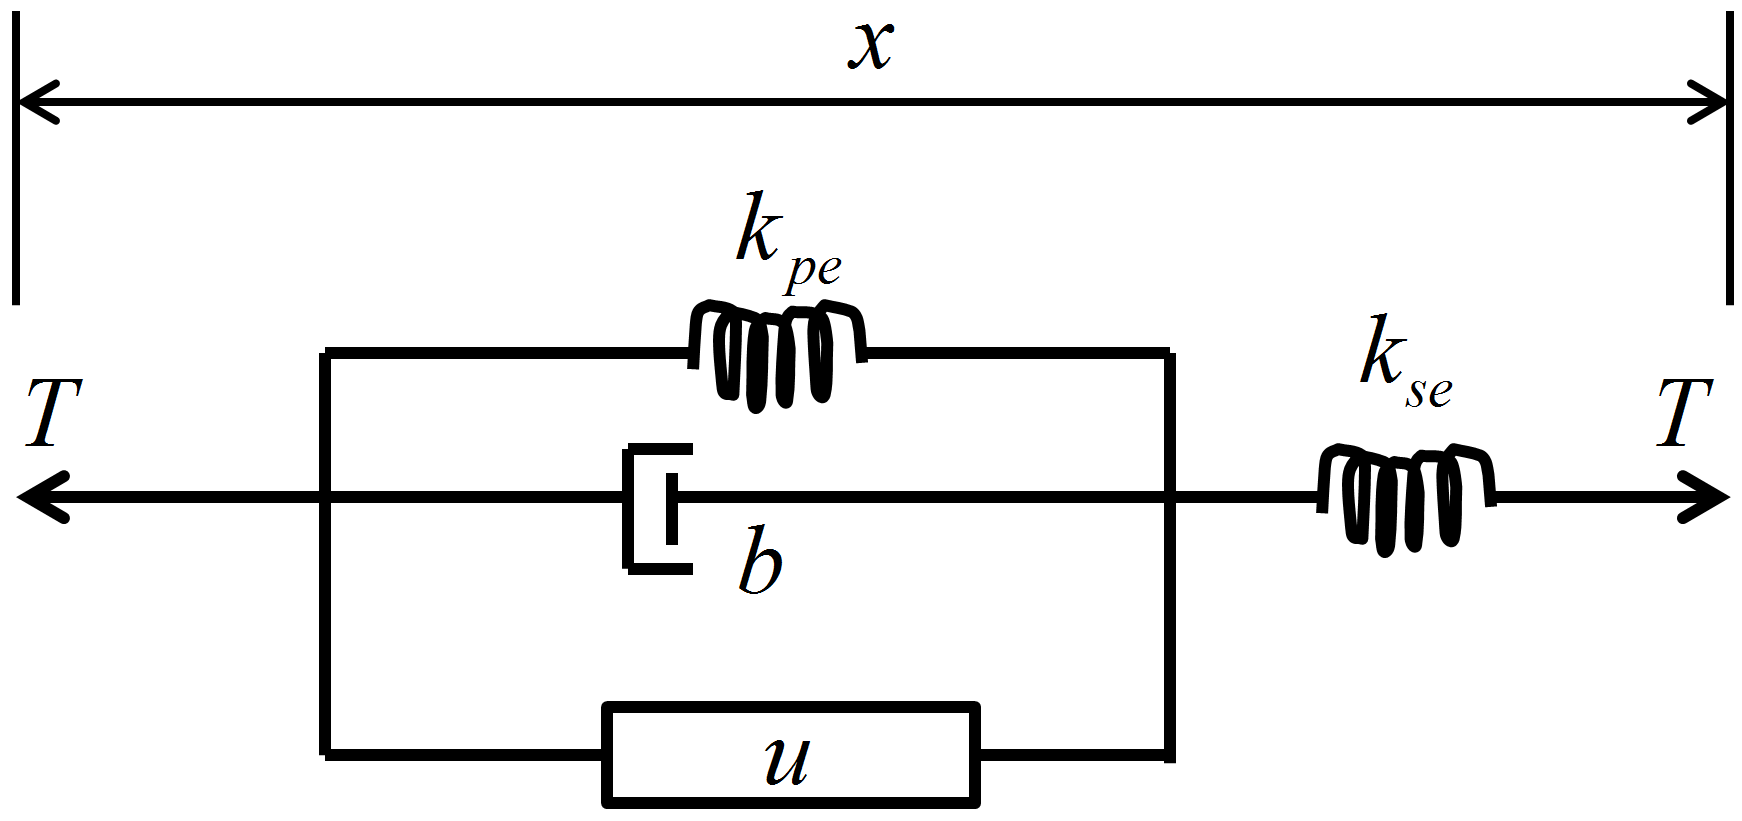
\includegraphics[width=2.75in]{musclemodel}
  \caption{Hill type muscle model}
\end{figure}

\noindent Basically, the model consists of two springs, a viscous damper and a actuation component.
The damper and one of the springs are connected in parallel and the other spring is
connected in serial. The active component in which our controller
can actuate resides in parallel side.
In real human body, many muscle fibers form bundles called \emph{fascicles}.
And multiple fascicles form a body of muscle.
To simplify our biped model, we use less than 10 muscle fibers to represent a certain kind of muscle body.
In the Hill type muscle model, we need four parameters for each:
a serial spring constant $k_{se}$, a parallel spring constant $k_{pe}$, a viscosity $b$ and a rest length $x_{r}$.
These parameters can be constants or variables depending on how muscle fibers modeled.
A mathematical expression defining dynamics of the muscle fiber is a first-order ordinary differential equation:
\begin{equation}\label{Tension}
\dot{T} = \frac{k_{se}}{b} \left( k_{pe}(x-x_{r})+b\dot{x}-\left(1+\frac{k_{pe}}{k_{se}}\right)T+u   \right)
\end{equation}
where $T$ is a tension exerted at both ends (positive means pulling), $x$ is the length of the fiber and $u$ is actuation force in the active component.
Note that all quantities shown in the equation are scalar values.
A muscle fiber always connects two rigid bodies and the same amount of
tension is applied to both of them with opposite directions.


There are muscle terminology to clearly define the configuration of muscles.
A muscle fiber has an $origin$ and an $insertion$ which indicate the attached position
of various muscle fibers at certain bones.
In other words, an origin and an insertion refer where a muscle fiber is originated from and inserted to, respectively.
If we denote the origin and insertion position of the fiber as $p_{org}$ and $p_{ins}$ in Cartesian coordinates,
the normalized direction of the fiber can be defined as $\hat{d}=(p_{ins}-p_{org})/||p_{ins}-p_{org}||$.
Thus, we can calculate tension $T\hat{d}$ and $-T\hat{d}$ which are applied to the origin and insertion body of the fiber, respectively.

We use two types of muscle fibers: actuated and unactuated muscle fibers.
Actuated muscle fibers represent the muscles we can actuate. Typically
they are attached to a middle of bones. Unactuated muscle fibers represent
ligaments around joints. We cannot deliberately actuate ligaments. Their
purpose is to maintain its rest length to prevent rigid bodies from
dislocations. For this reason, spring constants for ligaments are
comparatively larger than the actuated muscle fibers'.
In our system, the rest length of ligaments are configured to a small value.
This implies that the fiber length $||p_{ins}-p_{org}||$ happen to be zero
or near zero sometimes during simulation. In that case, we simply set
$x$ and $\dot{x}$ to zero.

An \emph{agonist}, or \emph{prime mover}, is a muscle whose contraction is chiefly responsible for producing a particular movement.
A muscle fibers has its \emph{antagonist}. The antagonist is a muscle whose action opposes that of a particular agonist.
We can choose specific muscle fibers to be used in the biped model based on agonists related to legs.
Also we can inform the optimizer to reduce actuation force on a muscle fiber when its antagonist is actively actuated.

\subsection{Soft joints}

Conventional biped models use reduced coordinates to represent a state.
They use a 6-DOF value on the root of the biped for position and orientation.
States for other bodies composing the biped have three or less DOFs with respect to joint types.
Since the other bodies have its own parent body, states are defined in the parent body local coordinates.
For instance, a calf has 1-DOF since its parent is a thigh and they are connected with a knee joint.
On the contrary, every body in the biped model we propose has a full 6-DOF to allow a slight joint dislocation.
In dynamics point of view, multiple rigid bodies are simulated individually without any joint constraints involved.
Without joint constraints, the pose of biped is not maintained occasionally due to a serious joint dislocation occurred during optimization process.
For instance, all bodies tend to collapse to the ground rather than preserving its normal pose when a high cost is given to the muscle fiber actuation.
By all means a certain human pose should be maintained and that is critically related to degrees of the joint dislocation.
We introduced a biomechanically-inspired ball joint to our biped model.
There are certain points defined in body coordinates on the bodies.
Two points came from two different bodies may form a soft joint.
The distance between two points should be constrained to $\epsilon$ or smaller where $\epsilon$ is a joint dislocation threshold.
To satisfy the constraints, we connect these two points with a stiff ligament fiber.
We assume that ligament fibers have no cost for actuation.
With these kind of joints, the biped can take advantages of shock absorption mechanism as well as prevention of joint dislocation.

\begin{figure}[h!]
  \centering
  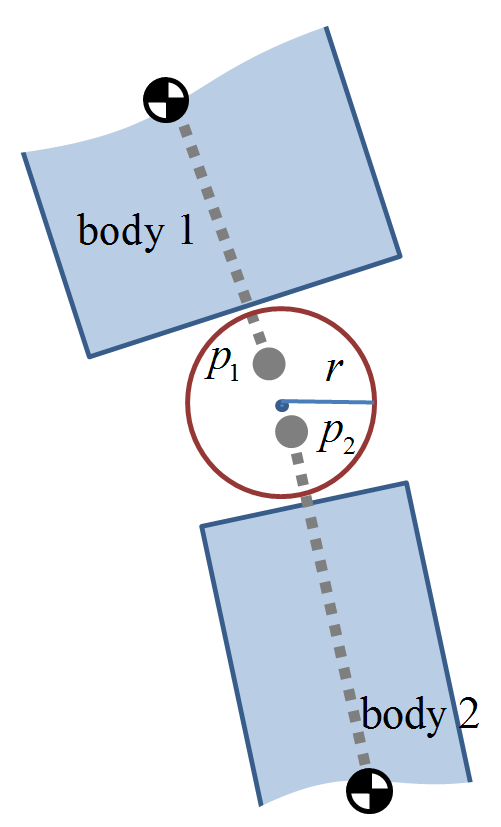
\includegraphics[width=1.5in]{softjoint}
  \caption{Structure of a soft joint}
\end{figure}


\subsection{Contact model}

There are various kind of techniques to deal with the calculation of contact forces between rigid bodies.
The existing algorithms can be divided into three categories: constraint-based, penalty-based and impulse-based approaches.
In constraint based methods, the contact forces are computed by solving an optimization problem such as linear complementarity problems (LCP).
The contact forces are calculated most precisely using LCP.
However, it is tricky to implement correctly and the solutions may not be found although they are exist or it is unsolvable in some cases \cite{StewartT00}.
These shortcomings are improved in \cite{Anitescu}.
They introduced a LCP formulation which guarantees that the contact problem always has a solution which will be found by Lemke's algorithm.
Penalty-based methods compute the contact forces by considering a contact as a spring-damper.
It is scalable and easy to implement. However it requires very short integration step especially at collisions and in most cases non-penetration conditions are violated.
Impulse-based methods model contacts as successive collisions instead of persisting contacts.

As long as the biped's poses are properly managed, our simulation configuration contains a relatively small number of contact points.
Contact forces are crucial because the root position and orientation of the biped can be controlled only by that forces.
Therefore physically conforming contact forces are important in the point of believable character animation.

We use a penalty method which can be easily integrated in our optimization framework.
The time-stepping method based on LCP is hard to combine with our quadratic programming (QP) formulation
because there is a case that LCP is not transformed into QP, \emph{i.e.},
a matrix involved in constraints is not a symmetric positive matrix.

A penalty method is a way to calculate contact normal forces with allowing a certain amount of penetration.
A temporary spring-damper element is created and attached where a contact is established.
The spring-damper exerts a strong force to separate two penetrated bodies.
After non-penetration constraints recovered the spring-damper is removed immediately.
Typically, a critically-damped spring is used to make the separation time minimal without oscillation.

\begin{figure}[h!]
  \centering
  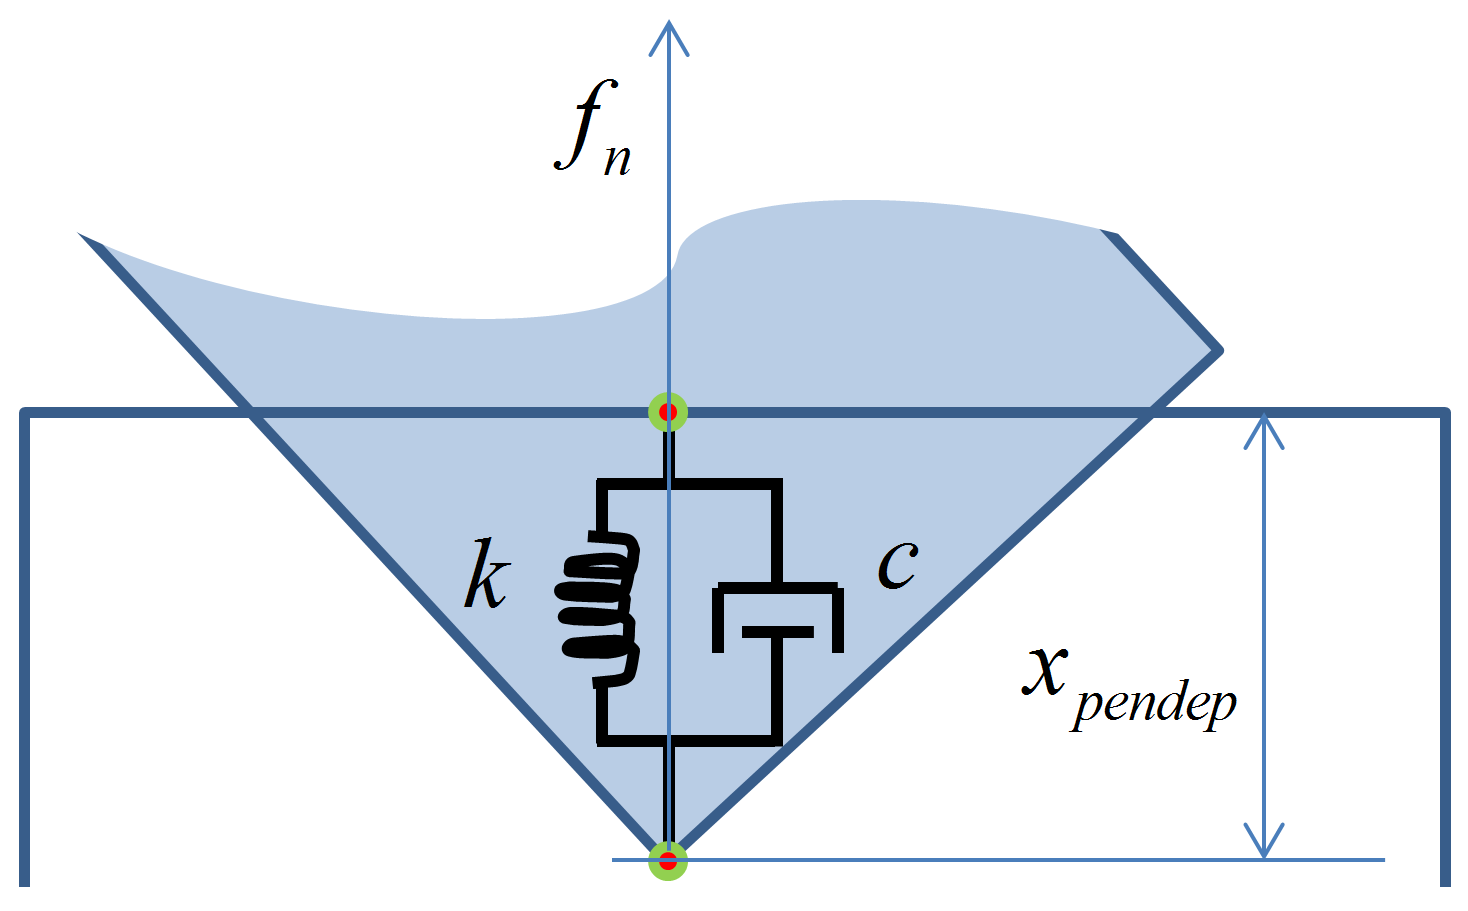
\includegraphics[width=2.5in]{penalty}
  \caption{Normal force calculated from the penalty method}
\end{figure}

Normal force exerted at the penetrated corner point of the box is calculated as follows:
\begin{equation}\label{penalty-normal}
f_n = -k x_{pendep} - c \dot{x}_{pendep}
\end{equation}
where $f_n$ is the normal force, $k$ is a spring constant, $c$ is a damping coefficient and $x_{pendep}$ is
a penetration depth. $k$ and $c$ is positive numbers and $x_{pendep}$ is a negative in case of penetration.
If a single rigid body of body mass $\bar{m}$ has $n_p$ contact points with the ground,
$n_p$ springs of the damping coefficient $c=2\sqrt{\bar{m}k/n_p}$ makes a critically damped system.

Since any normal force should be applied in unilateral manner, \emph{i.e.},
only pushing a penetrated body not pulling, we need an additional constraint $f_n \geq 0$.
$x_{pendep}$ will be always a negative scalar, so the term $-kx_{pendep}$ is always become a positive.
A problem arises when a penetrated corner point is in a separation phase,
especially when $kx_{pendep} < c\dot{x}_{pendep}$ which leads $f_n$ to a negative value.
To circumvent this issue, we add a nonnegative positive scalar term $\lambda$ to the right-hand side
of \eqref{penalty-normal} to obey the constraint $f_n \geq 0$. During optimization,
a minimal $\lambda$ to keep the constraint will be calculated
when we set a very high cost on that variable. We can denote \eqref{penalty-normal} with
discrete-time substitution that can be used as an equality constraint for the optimizer.
\begin{equation}\label{penalty-normal-discretized}
f_n = -k x_{pendep}^{(l+1)} - c \frac{x_{pendep}^{(l+1)} - x_{pendep}^{(l)}}{h} + \lambda
\end{equation}
Besides normal force, tangential contact force are needed to model friction.
Coulomb friction model is widely used.
There are two kinds of friction in this model: static friction and dynamic friction.
If contact points are sliding along the surface without breaking contacts,
dynamic friction force will act upon them. In this case, the friction force is depends
on the magnitude of normal force and velocity of sliding contact point along the surface.
Dynamic friction force $f_{tk}$ is
\begin{equation}\label{dynamic-friction}
f_{tk} = -\mu_k v |f_n|
\end{equation}
where $\mu_k$ is a coefficient of dynamic friction
and $v$ is velocity of sliding contact point along the surface.
On the other hand, static friction force occurs on a stationary contact point.
Contact force, that is sum of static friction and normal force, should lies on a cone
which is called Coulomb's friction cone.
It is allowed to choose any static friction force if the resulting contact force is
inside on the cone. We have two equations to express conditions of the static friction force:
\begin{equation}\label{static-friction}
\mu_s |f_n| \geq |f_{ts}|, \quad f_{ts} \cdot \hat{f}_n = 0
\end{equation}
where $f_{ts}$ is static friction force and $\mu_s$ is a coefficient of static friction.
Inner product equality implies that $f_{ts}$ should lies on the tangential space of contact point.

\subsection{Integration}
In general, controlled physical simulations are done in two steps.
First is to compute necessary forces or torques for control and
second is to integrate them to get a next state.
There are several integration techniques.
The most easy and intuitive one is an explicit Euler integration.
Most of rigid body systems can be simulated using an explicit Euler method
as far as there is no stiff component exists. The explicit integration
allows us a simple implementation and fast computation of a next state,
however, it has the potential of instability when the time step is larger
then a certain threshold. The threshold is mainly determined by a time
constant of a given differential equation we need to integrate.
In Euler method, next state is computed by the following equation:
\begin{equation}
Y^{(l+1)}=Y^{(l)} + hf(Y^{(l)}).
\end{equation}
where $h$ is an integration time step.
It is obvious that larger $h$ value will cause instability to the system.

On the contrary, an implicit integration does not suffer from this kind of
instability issue. The formula is like the following:
\begin{equation}
Y^{(l+1)}=Y^{(l)} + hf(Y^{(l+1)}).
\end{equation}
That is, we want to find the next state $Y^{(l+1)}$ where we
reverse the time step by $-h$ from $Y^{(l+1)}$, we get to the current state
$Y^{(l)}$. In most cases, $f$ is a nonlinear function of $Y$, so we need to
linearize it to find closed form solution of $Y^{(l+1)}$. If we define a
variable $\Delta Y = Y^{(l+1)}-Y^{(l)}$, it can be calculated using the
following equation:
\begin{equation}\label{DeltaY}
\Delta Y = \left(  \frac{1}{h}\mathbf{1} - {\frac{\partial f}{\partial Y} \bigg|_{Y=Y^{(l)}}}\right)^{-1} f(Y^{(l)})
\end{equation}
where $\mathbf{1}$ is an identity matrix. We need an analytic form of
Jacobian $\partial f / \partial Y$ to calculate $\Delta Y$.

In our case, the time constant is dominated by muscle fibers because they consists
of highly stiff springs \eqref{Tension}. Even if we use a small time step
such as $h=0.01$, our system occasionally diverges slowly with the explicit Euler
integration. Therefore, it is obvious that the implicit integration scheme is right one to choose.
Unfortunately, it is not suitable for our simulation framework because
the control part and the integration part is combined into a single linear equation in our case.
Since $\Delta Y$ is not a linear function of $Y^{(l)}$, the implicit integration approach
is hard to be combined into our framework. For a compromise, we employed the explicit Euler
with very small time step.

\section{Putting it all together}
By gathering all equality and inequality constraints introduced so far,
we get the following optimization formulation.

minimize
\begin{equation}\notag
w_{ref} || \chi^{(l+1)} - \chi^{(l+1)}_{ref} || +
w_{com} || p^{(l+1)}_{com} - p^{(l+1)}_{com,ref} || + w_u || u ||
\end{equation}
subject to
\begin{align}
\chi^{(l+1)} &= \tilde{M}^{-1} (f_f + f_c + f_g + f_{ext} - \tilde{C})          &                        \notag   \\
f_{f_i}      &= (A_i u_i + B_i x_i^* + C_i) \frac{b_i - a_i}{ || b_i - a_i || } & i \in \mathcal{M}      \notag   \\
f_{c,i}      &= f_{n,i} + f_{tk, i}                                             & i \in \mathcal{P}_k    \notag   \\
f_{c,i}      &= f_{n,i} + f_{ts, i}                                             & i \in \mathcal{P}_s    \notag   \\
r_i          &\geq || Z_i \chi^{(l+1)} + V_i ||                                 & i \in \mathcal{J}      \notag
\end{align}
The optimizer tries to find the solution, next state $\chi^{(l+1)}$, which is
close to $\chi^{(l+1)}_{ref}$ provided from motion clip with minimal effort.
Deviation cost for COM is added as a cost term to give more importance on COM tracking.
The solution should satisfy four types of constraints:
equations of motion, muscle forces, contact forces, soft joints.
Optimization variables excluding dependent variables are $u$, $x^*$ and $f_{ts}$.
Solving the optimization problem is done for frame by frame.
After next state $\chi^{(l+1)}$ is calculated, current state is updated to
next state and the frame counter $l$ is increased by 1.

Balancing the walking robot is very important.
Technically speaking, if a ground-projected COM lies
in biped's support polygon, the biped can manage to sustain
its balance. If COM is not lied inside support polygon,
bipeds will fall down no matter how hard they try not to
fall down.
Confining projected COM in support polygon
using additional optimization constraints seem to be
an intuitive way for solving this issue, but that kind
of approach results in robot-like stiff motion.

We used a slightly modified version of support polygon
to allow COM lies in outside of support polygon.
The modified support polygon is defined as a convex hull of
ground-projected corner points of sole and toe bodies.
We set $p_{com,ref}^{(l+1)}$ to the center of the modified
support polygon. And a constraint
$r_{sp} \geq || p^{(l+1)}_{com} - p^{(l+1)}_{com,ref} ||$
added to guarantee that COM is confined inside the modified
support polygon where $r_{sp}$ is a distance between the
center of modified support polygon and a point closest to
the center on the boundary of that polygon.

\section{Result}
We used a commercial optimization solver MOSEK to solve
the optimization problem.
About 300 muscle fibers are selected and attached to
rigid bodies composing the biped.
The complexity of optimization problem is mainly
dependent on the number of rigid bodies, muscle fibers, soft joints
and contact points. Except contact points, every components
constructing the biped is the same for the whole simulation process,
optimization solving performance is slightly varied with respect
to the number of contact points. In average, the solver takes
about 0.1 second for each frame.

Various simulation frequency from 30 Hz to 1 kHz
are tested. To achieve real-time performance,
large time step is desired. Since we used
a penalty-based contact force calculation, small
time step is required to maintain simulation stability.
We used ground spring constant $k=50000 N/m$ and
in this case, 300 Hz is sufficient for a stable simulation.

There are a lot of parameters to tune. The most
predominant factors are weights on the cost function.
For instance, if we suppress actuation force by increasing $w_u$
the biped will move limply. Weights should be taken with care since
exceedingly large weights on a certain term will results in
tendency to ignore remaining terms.

Muscle fiber parameters can be varied to get various motions.
For example, a high $k_{se}$ gives more robot-like movement while a low value
gives human-like elastic motion. However, viscous damping constant
$b$ does not play a significant role in making various motions.

Employing soft joints instead of rigid joints makes a resilient
feature on bipeds when external disturbance is applied.
With rigid joints, external force acting on a segment of biped
will affect every body segment because they are connected with
one or more rigid joints. On the other hand, in our model,
external force in a certain range on a body segment will only
affect on that body by allowing a little dislocation on joints.

\section{Conclusions}
In this paper, we introduced a simple but new concept to
conventional biped model to synthesize character animation.
Parameters regarding to soft joints and muscle fibers have
not been used in previous biped models at all.
By tweaking model parameters, we synthesized various human
motions based on motion capture data.

As future work, a more sophisticated balance strategy is
considered. For example, we want to automatically decide
where a foot should be placed to maintain its balance
when a very strong force is applied to the biped
without any forewarning.

%
% The following two commands are all you need in the
% initial runs of your .tex file to
% produce the bibliography for the citations in your paper.
\bibliographystyle{abbrv}
\bibliography{muscle}  % sigproc.bib is the name of the Bibliography in this case
% You must have a proper ".bib" file
%  and remember to run:
% latex bibtex latex latex
% to resolve all references
%
% ACM needs 'a single self-contained file'!
%
%APPENDICES are optional
%\balancecolumns
%\appendix
%Appendix A

\balancecolumns
% That's all folks!
\end{document}
